% chktex-file 1
% chktex-file 2
% chktex-file 3
% chktex-file 8
% chktex-file 13
% chktex-file 24
% chktex-file 40
% chktex-file 44
\documentclass[pdflatex,sn-nature]{sn-jnl}

\setcitestyle{numbers,comma,sort,open={},close={}}

\makeatletter
\renewcommand\cite[1]{\unskip\textsuperscript{\citep{#1}}}
\makeatother

\hbadness=10000
\vbadness=10000
\vfuzz=10pt
\hypersetup{hypertexnames=false}

%%%% User-added packages
\usepackage[left]{lineno}
\usepackage[utf8]{inputenc}
\usepackage[T1]{fontenc}
\usepackage{siunitx}
\usepackage{hyperref}
\usepackage{makecell}

%%%% Standard Packages
%%<additional latex packages if required can be included here>
\usepackage{graphicx}%
\usepackage{multirow}%
\usepackage{amsmath,amssymb,amsfonts}%
\usepackage{amsthm}%
\usepackage[title]{appendix}%
\usepackage{xcolor}%
\usepackage{textcomp}%
\usepackage{manyfoot}%
\usepackage{booktabs}%
\usepackage{algorithm}%
\usepackage{algorithmicx}%
\usepackage{algpseudocode}%
\usepackage{listings}%

%%%% User-added
%%%%%%%%%%%%%%%% 색상 %%%%%%%%%%%%%%%%

% 색상 확장
\usepackage[dvipsnames,table]{xcolor}

\usepackage{color}
\definecolor{BLACK-COLOR}{rgb}{0,0,0}

\definecolor{ORANGE-COLOR}{rgb}{1,0.5,0}
\newcommand{\orange}{\color{ORANGE-COLOR}}
\definecolor{BLUE-COLOR}{rgb}{0,0.25,1}
\newcommand{\blue}{\color{BLUE-COLOR}}
\definecolor{RED-COLOR}{rgb}{1,0.25,0}
\newcommand{\red}{\color{RED-COLOR}}
\definecolor{YELLOW-COLOR}{rgb}{1,1,0.1}
\newcommand{\yellow}{\color{YELLOW-COLOR}}
\definecolor{GREEN-COLOR}{rgb}{0.1,0.9,0.3}
\newcommand{\green}{\color{GREEN-COLOR}}
\definecolor{PURPLE-COLOR}{rgb}{0.57,0,0.82}
\newcommand{\purple}{\color{PURPLE-COLOR}}
\definecolor{WHIE-COLOR}{rgb}{1,1,1}
\newcommand{\white}{\color{WHIE-COLOR}}
\definecolor{DARKGREEN-COLOR}{rgb}{0.29,0.49,0.27}
\newcommand{\darkgreen}{\color{DARKGREEN-COLOR}}
\definecolor{CRIMSON-COLOR}{rgb}{0.6,0,0}
\newcommand{\crimson}{\color{CRIMSON-COLOR}}

\definecolor{DARKBLUE-COLOR}{rgb}{0.0, 0.0, 0.75}
% \newcommand{\darkblue}{\color{DARKBLUE-COLOR}}
\newcommand{\darkblue}{\color{CRIMSON-COLOR}}
%\newcommand{\darkblue}{\color{BLACK-COLOR}}

\newcommand{\greennoshow}{\color{BLACK-COLOR}}
\newcommand{\darkgreennoshow}{\color{BLACK-COLOR}}
\newcommand{\rednoshow}{\color{BLACK-COLOR}}
\newcommand{\purplenoshow}{\color{BLACK-COLOR}}


\usepackage{comment}

\newcommand\marklessfootnote[1]{
    \addtocounter{footnote}{1} %no call is made to \footnotemark.
    \footnotetext{#1}
}







%======================
%  Front Matter
%======================

\begin{document}
\linenumbers

\title{A post-hoc codon-accessibility regularizer for calibrating protein language models without retraining}

\author[1,2]{Hyoseok Jang${}^{\ast}{}^{,}\hspace{-1.5em}$
\marklessfootnote{Equally contributed.}.
}
\author[1]{Sangchul Lee${}^{\ast}{}^{,}$}
\author[3]{David S. Yang${}^{\ast}{}^{,}$}
\author[4]{Haneol Cho}
\author[3,5]{Cherlhyun Jeong${}^{\dagger}{}^{,}$}
\author[1,2]{Chansoo Kim${}^{\dagger}{}^{,}\hspace{-1.25em}$
\marklessfootnote{Correspondence should be addressed to \href{mailto:che.jeong@kist.re.kr}{che.jeong@kist.re.kr} and \href{mailto:eau@ust.ac.kr}{eau@ust.ac.kr}.}
}

\date{}
\affil[1]{Computational Science Research Center, Korea Institute of Science and Technology (KIST), Seoul 02792, Republic of Korea}
\affil[2]{AI-Robot Department, University of Science and Technology (UST), Seoul 02792, Republic of Korea}
\affil[3]{Chemical and Biological Integrative Research Center, Korea Institute of Science and Technology, Seoul 02792, Republic of Korea}
\affil[4]{Computer Science and Engineering, Sejong University, Seoul 05006, Republic of Korea}
\affil[5]{Division of Bio-Medical Science \& Technology, University of Science and Technology, Seoul 02792, Republic of Korea}

% \affil[$\dagger$]{Equally contributed}
% \affil[$\ast$]{Correnspondence should be addressed to \mailto{che.jeong@kist.re.kr}{che.jeong@kist.re.kr} and \mailto{eau@ust.ac.kr}{eau@ust.ac.kr}}






%%%%%%%%%%%%%%%%%%%%%%%%%%%% abstract
\abstract{
Viruses escape host immunity through rapid evolution, challenging genomic surveillance and vaccine design. Protein language models (PLMs) capture amino-acid–level functional constraints, but typically ignore nucleotide-level mutation processes that determine which substitutions are genetically reachable. We present codon-aware constrained semantic change (CAC), a post-hoc calibration framework that couples any PLM with CLIMB, a codon-transition Markov regularizer that scores the accessibility of amino-acid substitutions under nucleotide mutation biases. CAC augments protein-level semantic-change and grammaticality scores with an explicit accessibility prior, correcting amino-acid–only objectives without retraining, fine-tuning, or access to model internals. This plug-and-play design enables fast, low-cost upgrades of existing PLM-based predictors and improves portability across model families. Applied to SARS-CoV-2, CAC consistently improves escape-pathway prediction across diverse PLM architectures, including general-purpose ESM-2 models, yielding up to a 44\% improvement in mean rank (from 9,130 to 5,037 among 24,187 candidates). In addition, CAC reveals a time-scale–dependent shift in the dominant signals—from codon accessibility at short horizons to protein-level constraints at longer horizons—consistent with established evolutionary dynamics.
}






\maketitle










%%%%%%%%%%%%%%%%%%%%%%%%%%%% article

\section*{Introduction}

Predicting how viruses evolve under immune pressure is a central problem in computational biology with direct implications for surveillance, vaccine design, and preparedness. Recent progress in protein language models (PLMs) has enabled sequence-based prediction without explicit structural modeling, motivating a view of viral evolution as a language problem. In this framing, viral fitness corresponds to a form of “grammaticality,” while immune escape corresponds to “semantic change,” and variants are prioritized by trading off these two objectives.

A representative approach, constrained semantic change search (CSCS), operationalizes this idea by identifying mutations that preserve fitness (high grammaticality) while inducing antigenic novelty (high semantic change), and has shown strong performance for RNA viruses. However, despite these successes, current PLM-based predictors optimize and score candidates purely in amino-acid space, implicitly treating amino-acid substitutions as equally reachable proposals subject only to protein-level constraints.

From a computational-science perspective, this introduces a systematic model–process mismatch: the phenotype is evaluated at the protein level, but the generative mechanism of variation is governed by the nucleotide code. In practice, mutational events are shaped by codon-to-codon transition biases and by the availability of single-nucleotide pathways, so that some amino-acid substitutions are substantially more probable than others even before selection. Ignoring this accessibility layer amounts to optimizing an objective with a missing feasibility prior (or regularization term), which can distort ranking by overemphasizing protein-level scores for substitutions that are genetically unlikely while underweighting substitutions favored by common nucleotide transitions.

Here, we introduce CLIMB, a lightweight nucleotide-level scoring term that quantifies the accessibility of an amino-acid substitution under a codon-transition process. We integrate CLIMB into the CSCS framework to create codon-aware constrained semantic change (CAC) search, a unified scoring scheme that combines (i) amino-acid semantic change, (ii) amino-acid grammaticality, and (iii) nucleotide-driven mutational accessibility as explicit, separately weighted terms. Crucially, CLIMB is model-agnostic: it can be attached as a plug-and-play post-hoc module to calibrate any existing or future PLM—ranging from specialized viral predictors to general-purpose foundation models—without retraining, fine-tuning, or access to model internals. This design addresses a practical bottleneck in deploying PLMs for biological forecasting: improvements typically require expensive, model-specific modification, whereas CAC provides a low-cost, portable correction that injects nucleotide-level feasibility into protein-level ranking.

We validate CAC across four distinct PLM architectures, including the original CSCS BiLSTM model and multiple ESM-2 family models, using extensive deep mutational scanning measurements and mutations observed in major variants of concern. Across settings, incorporating codon accessibility consistently improves escape prediction, with gains of up to 44\% and the largest benefits when calibrating large general-purpose foundation models. Moreover, at short horizons, nucleotide substitution rates dominate and prioritize genetically accessible mutations. Over longer horizons, protein-level constraints dominate, and rankings increasingly reflect amino-acid–level compatibility. This trend is consistent with known features of evolutionary trajectories.
\smallskip

\noindent\textbf{Contributions.} This work provides (1) a codon-aware calibration term (CLIMB) that augments amino-acid–only objectives with a nucleotide-level feasibility prior; (2) a model-agnostic CAC framework that upgrades existing PLM-based predictors via simple post-hoc integration; and (3) systematic validation across architectures and datasets, together with an analysis of time-scale–dependent weight shifts that links model behavior to known evolutionary patterns.

% === Figure 1: 기존 코드를 그대로 유지 ===
\begin{figure}[t]
   \centering
   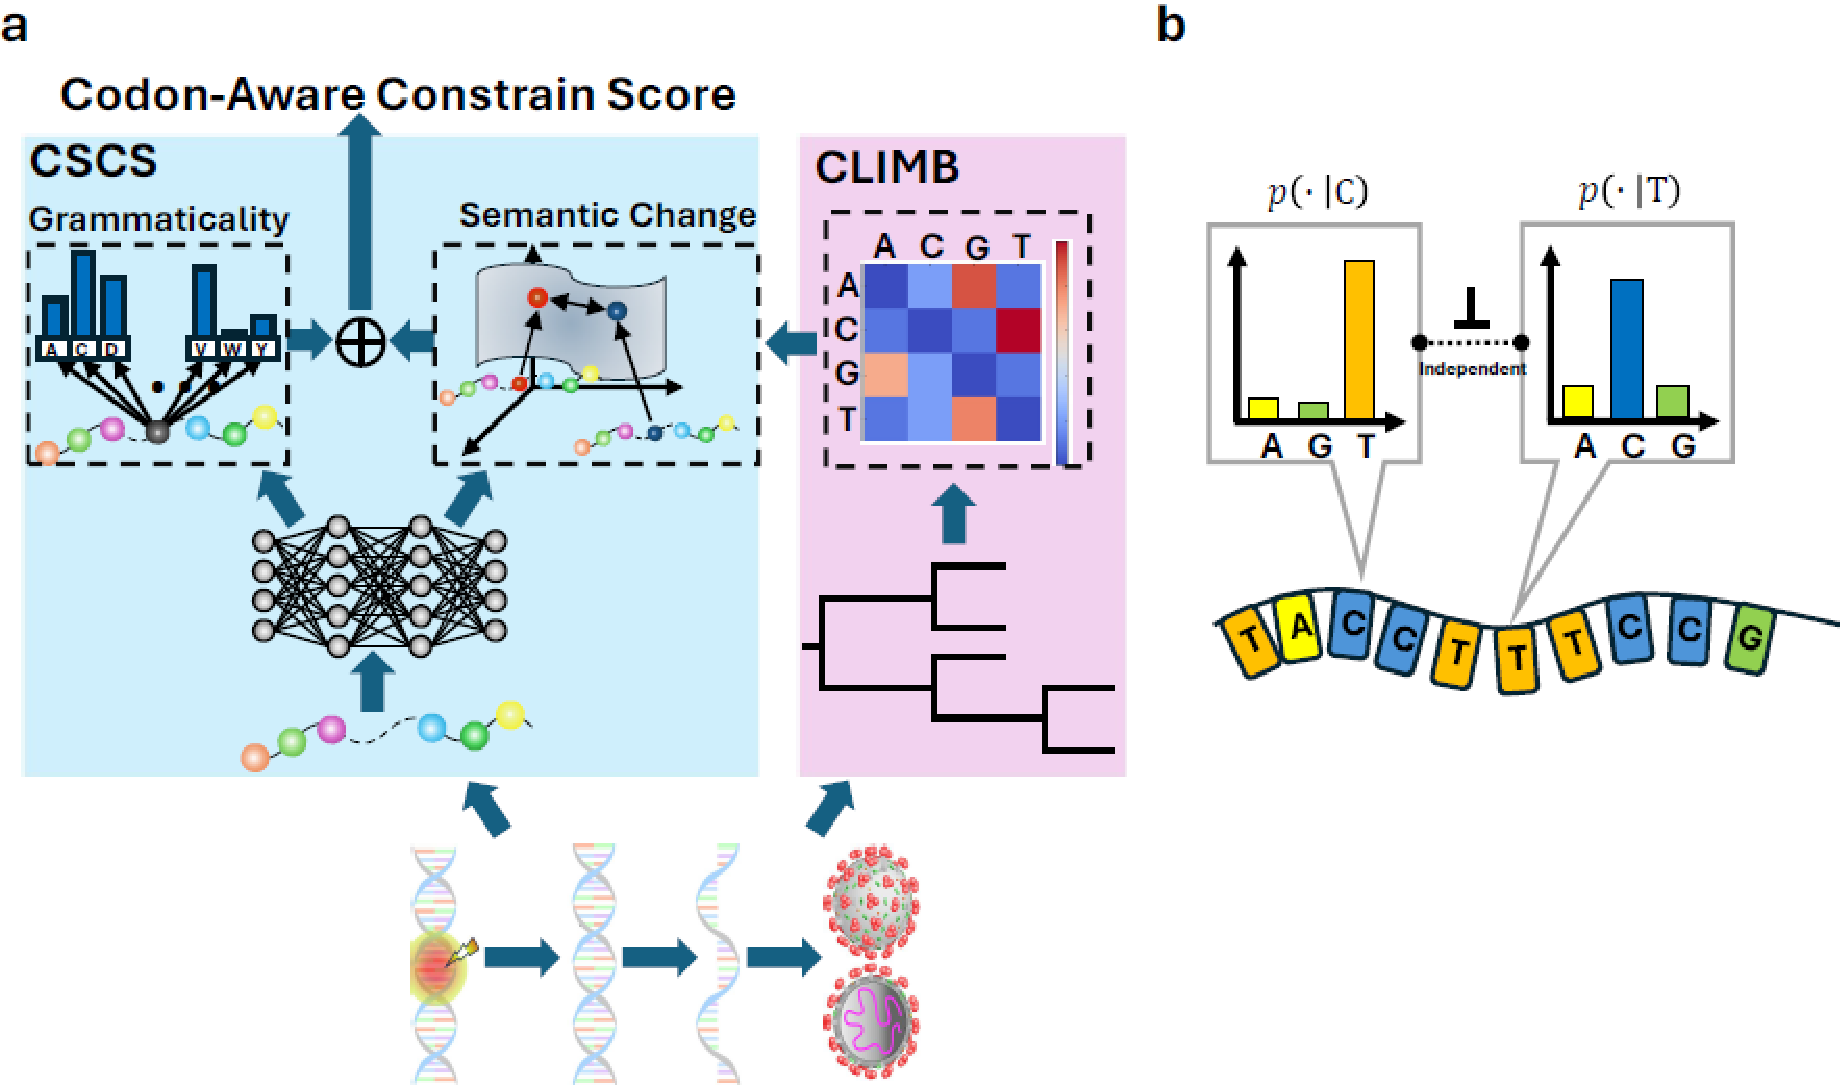
\includegraphics[width=\linewidth]{Figure_Nature_1.pdf} % 실제 파일명으로 교체 필요
   \caption{
       \textbf{Conceptual framework for integrating codon-level mutational biases with protein language models.}
       (\textbf{a}) Schematic of the codon-aware constrained semantic change search (CAC) model. The CAC score is generated by synergistically combining two distinct information streams. The first is derived from a protein language model (PLM), which computes the protein-level grammaticality ($\mathrm{s}_\text{g}$) and semantic change ($\mathrm{s}_\text{s}$) for a given mutation. The second is our proposed nucleotide-level codon likelihood Markov bias regularizer, CLIMB ($\mathrm{s}_\text{p}$), derived from phylogenetic reconstruction. CLIMB uses an estimated nucleotide transition rate matrix ($\mathbf{Q}$) to quantify the inherent mutational biases governing viral evolution. The final CAC score is a weighted combination of these components.
       (\textbf{b}) Illustration of the nucleotide-level mutational biases captured by the CLIMB regularizer. The probability of a base mutating to any other base is not uniform. For example, the observed mutational spectrum of SARS-CoV-2 shows a high propensity for C$\to$T transitions (left plot), while transitions from T are distributed more evenly (right plot). The CLIMB score quantifies the likelihood of all possible amino acid substitutions by considering the probabilities of the underlying codon-to-codon mutation pathways.
   }
  \label{fig:1}
\end{figure}





%%%%%%%%%% Results %%%%%%%%%%
\section*{Results}

\subsection*{Post-hoc codon-transition calibration yields universal gains in escape prediction across PLM backbones}

\begin{figure}[t]
    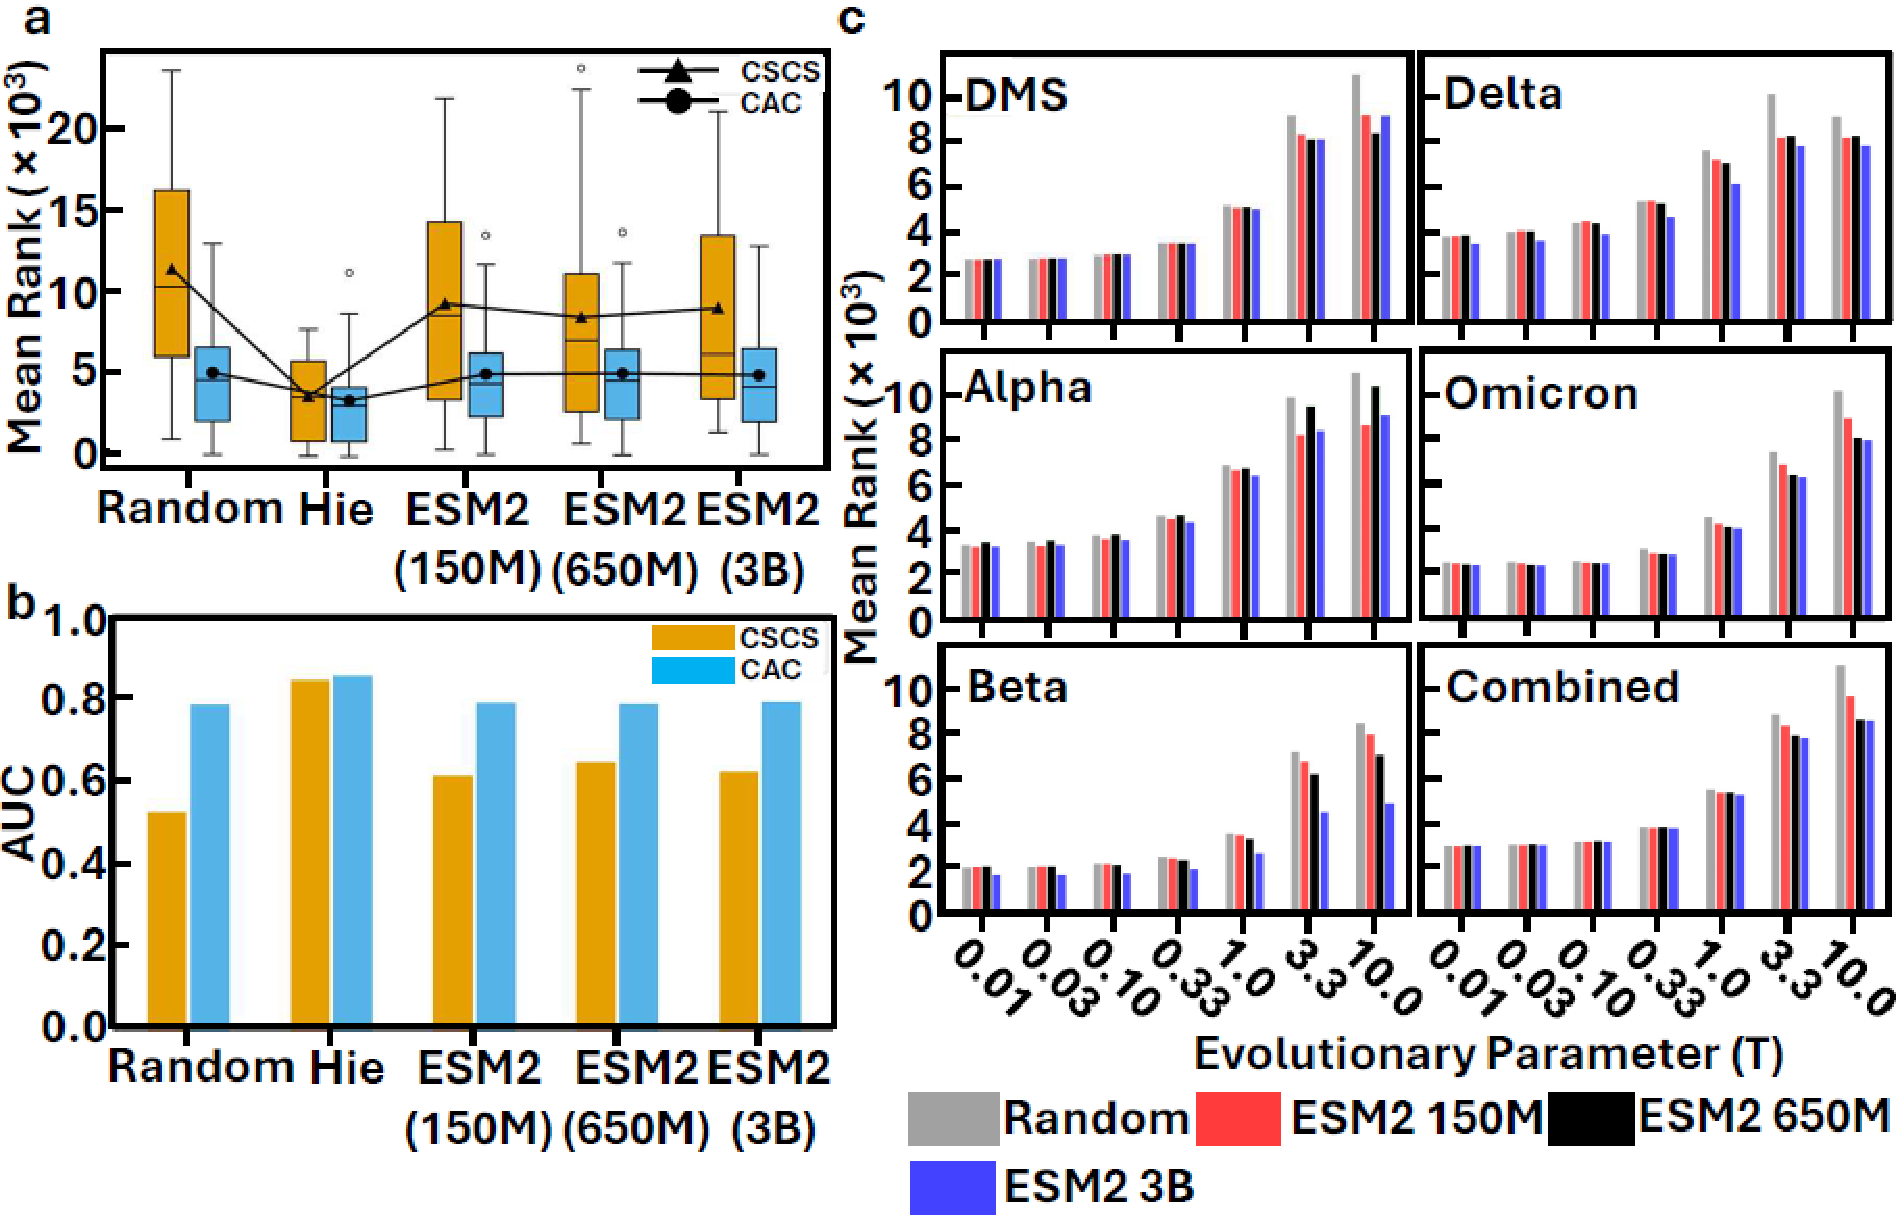
\includegraphics[width=\linewidth]{Figure_Nature_2.pdf}
    \caption{
    \textbf{Integration of codon-level information robustly improves viral escape prediction.}
    %
    Predictive performance of the full CAC model compared to the baseline CSCS, an ablation control (CLIMB-only), and a random baseline across various protein language model (PLM) backbones.
    We evaluate their performance on known SARS-CoV-2 escape mutations using two metrics: mean rank (lower is better) and area under the curve (AUC; higher is better).
    %
    (\textbf{a}) Box plots comparing the distribution of escape mutation ranks from the DMS validation set for CAC (green) and CSCS (blue).
    The central line indicates the median, the box represents the interquartile range, and the solid dot/triangle shows the mean.
    %
    (\textbf{b}) Comparison of AUC values for escape prediction. CAC consistently achieves a higher AUC than the CSCS baseline across all model backbones.
    %
    (\textbf{c}) Mean escape rank for CAC as a function of the evolutionary timescale parameter, $T$, for different ESM-2 models across six validation sets.
    %
    These plots illustrate the effect of model size and evolutionary context on predictive performance, with larger models often showing greater performance gains.
    }
    \label{fig:2}
\end{figure}

The CAC method delivers substantial and largely significant improvements in viral escape prediction over the baseline CSCS method, as tested across multiple PLM backbones on six SARS-CoV-2 validation sets (DMS, Alpha, Beta, Delta, Omicron, and Combined).
These results support the central premise that injecting a codon-transition prior—a lightweight mutation-process term—as a post-hoc calibration of amino-acid–level PLM scores can systematically improve escape prioritization without retraining or fine-tuning the backbone model.

% For example, on the DMS validation set for the Wuhan-Hu-1 spike protein~\cite{baum2020antibody}, CAC method yield its most substantial enhancements, when applied to large generalist models.
% This approach dramatically improve the performance of the ESM-2-3B model, reducing the mean escape rank from $9130 \pm 6500$ (mean $\pm$ s.d.) to $5037 \pm 3586$.
% The improvement is statistically significant (Wilcoxon signed-rank test, $p = 0.0031$).
% Similar significant gains are observed for the ESM-2-150M and ESM-2-650M models (Table~\ref{tab:cac_vs_cscs} and Fig.~\ref{fig:2}a).

For instance, on the DMS validation set for the Wuhan-Hu-1 spike protein~\cite{baum2020antibody}, CAC yields its most substantial gains when calibrating large, general-purpose models. For ESM-2-3B, CAC reduces the mean escape rank from $9130 \pm 6500$ (mean $\pm$ s.d.) to $5037 \pm 3586$, a statistically significant improvement (one-sided Wilcoxon signed-rank test, $p = 0.0031$). Similar significant gains are observed for ESM-2-150M and ESM-2-650M (Table~\ref{tab:cac_vs_cscs}, Fig.~\ref{fig:2}a).

% Interestingly, even though the specialized Hie-BiLSTM model also showed a slight improvement in mean rank (from $3757$ to $3493$), this difference is not statistically significant on this validation set ($p = 0.55$).
% It implies that the predictive benefit of integrating codon-level constraints is most pronounced when synergizing with the broad sequence understanding of large-scale generalist PLMs.

In contrast, the specialized Hie-BiLSTM backbone shows a smaller and non-significant improvement on this particular validation set (mean rank $3757$ to $3493$, $p=0.55$). One interpretation is that specialized viral models may already partially reflect short-horizon substitution tendencies, leaving less room for additional post-hoc calibration, whereas large general-purpose PLMs benefit more strongly from an explicit mutation-process prior.


\begin{table}[htbp]
    \centering
    \caption{\textbf{Escape mean ranks for various model backbones and scoring methods.} This table compares the predictive performance of the codon-aware
    %constrained semantic change search (CAC)
    CAC
    method against the baseline
    %constrained semantic change search (CSCS)
    CSCS
    across several protein language model backbones.
    Its performance is quantified as the mean rank of known escape mutations, where a lower rank indicates better predictive power.
    The CAC scores are reported using an evolutionary timescale parameter of $T=1$.
    Statistical significance of the improvement by CAC over CSCS is determined using a one-sided Wilcoxon signed-rank test.
    Across all tested model architectures and validation sets, the CAC method consistently achieves a lower mean rank than the baseline CSCS.
    See Supplementary Table S1 for details of the validation sets.}
    \begin{tabular}{c|c|c|c|c}
        \toprule
        \multirow{2}[2]{*}{\bfseries \makecell{Validation \\ set}}
        & \multirow{2}[2]{*}{\bfseries \makecell{Model \\ backbone}}
        & \multicolumn{2}{c|}{\bfseries Escape rank (mean $\pm$ s.d.)}
        & \multirow{2}[2]{*}{\bfseries \makecell{Significance \\ ($p$-value)}}
        \\
        \cmidrule{3-4}
        % multirow
        & % multirow
        & \bfseries CSCS baseline
        & \bfseries CAC
        &
        \\
        %
        % DMS validation set
        %
        \midrule
        \midrule
        DMS
        & Hie-BiLSTM
        & 3757 $\pm$ 2574
        & 3493 $\pm$ 2974
        & $0.55$
        %
        \\
        \cmidrule{2-5}
        & ESM-2-150M
        & 9387 $\pm$ 6127
        & 5098 $\pm$ 3667
        & $6.2 \times 10^{-3}$
        \\
        \cmidrule{2-5}
        & ESM-2-650M
        & 8562 $\pm$ 6870
        & 5143 $\pm$ 3701
        & $1.3 \times 10^{-2}$
        \\
        \cmidrule{2-5}
        & ESM-2-3B
        & 9130 $\pm$ 6500
        & 5037 $\pm$ 3586
        & $3.1 \times 10^{-3}$
        \\
        %
        % Combined validation set
        %
        \midrule
        \midrule
        Combined
        & Hie-BiLSTM
        & 6260 $\pm$ 5378
        & 3841 $\pm$ 4184
        & $2.4 \times 10^{-4}$
        \\
        \cmidrule{2-5}
        & ESM-2-150M
        & 9816 $\pm$ 6053
        & 5309 $\pm$ 4280
        & $1.3 \times 10^{-6}$
        \\
        \cmidrule{2-5}
        & ESM-2-650M
        & 8857 $\pm$ 6263
        & 5327 $\pm$ 4196
        & $1.6 \times 10^{-5}$
        \\
        \cmidrule{2-5}
        & ESM-2-3B
        & 8736 $\pm$ 6095
        & 5204 $\pm$ 4054
        & $8.6 \times 10^{-6}$
        \\
        \bottomrule
    \end{tabular}
    \label{tab:cac_vs_cscs}
\end{table}

% Performance enhancement is consistently observe across all model architectures.
% In particular, within the ESM-2 family, we also observe a general relationship between increased model size and better performance gains across multiple validation sets (Fig.~\ref{fig:2}c).
% This scaling behavior is most pronounced for the Delta variant validation set, where ESM-2-3B achieves optimal performance within the ESM-2 family ($6154$, mean rank), outperforming both ESM-2-650M ($7094$) and ESM-2-150M ($7255$).

This enhancement is consistently observed across model architectures and validation sets. Within the ESM-2 family, we also observe a general scaling trend in which larger models exhibit larger performance gains in multiple settings (Fig.~\ref{fig:2}c). This scaling behavior is most pronounced for the Delta variant validation set, where ESM-2-3B achieves the optimal performance within the ESM-2 family (mean rank $6154$), outperforming ESM-2-650M ($7094$) and ESM-2-150M ($7255$).


\subsection*{Nucleotide mutation biases serve as a potent independent evolutionary prior across pandemic variants}

\begin{figure}[t]
    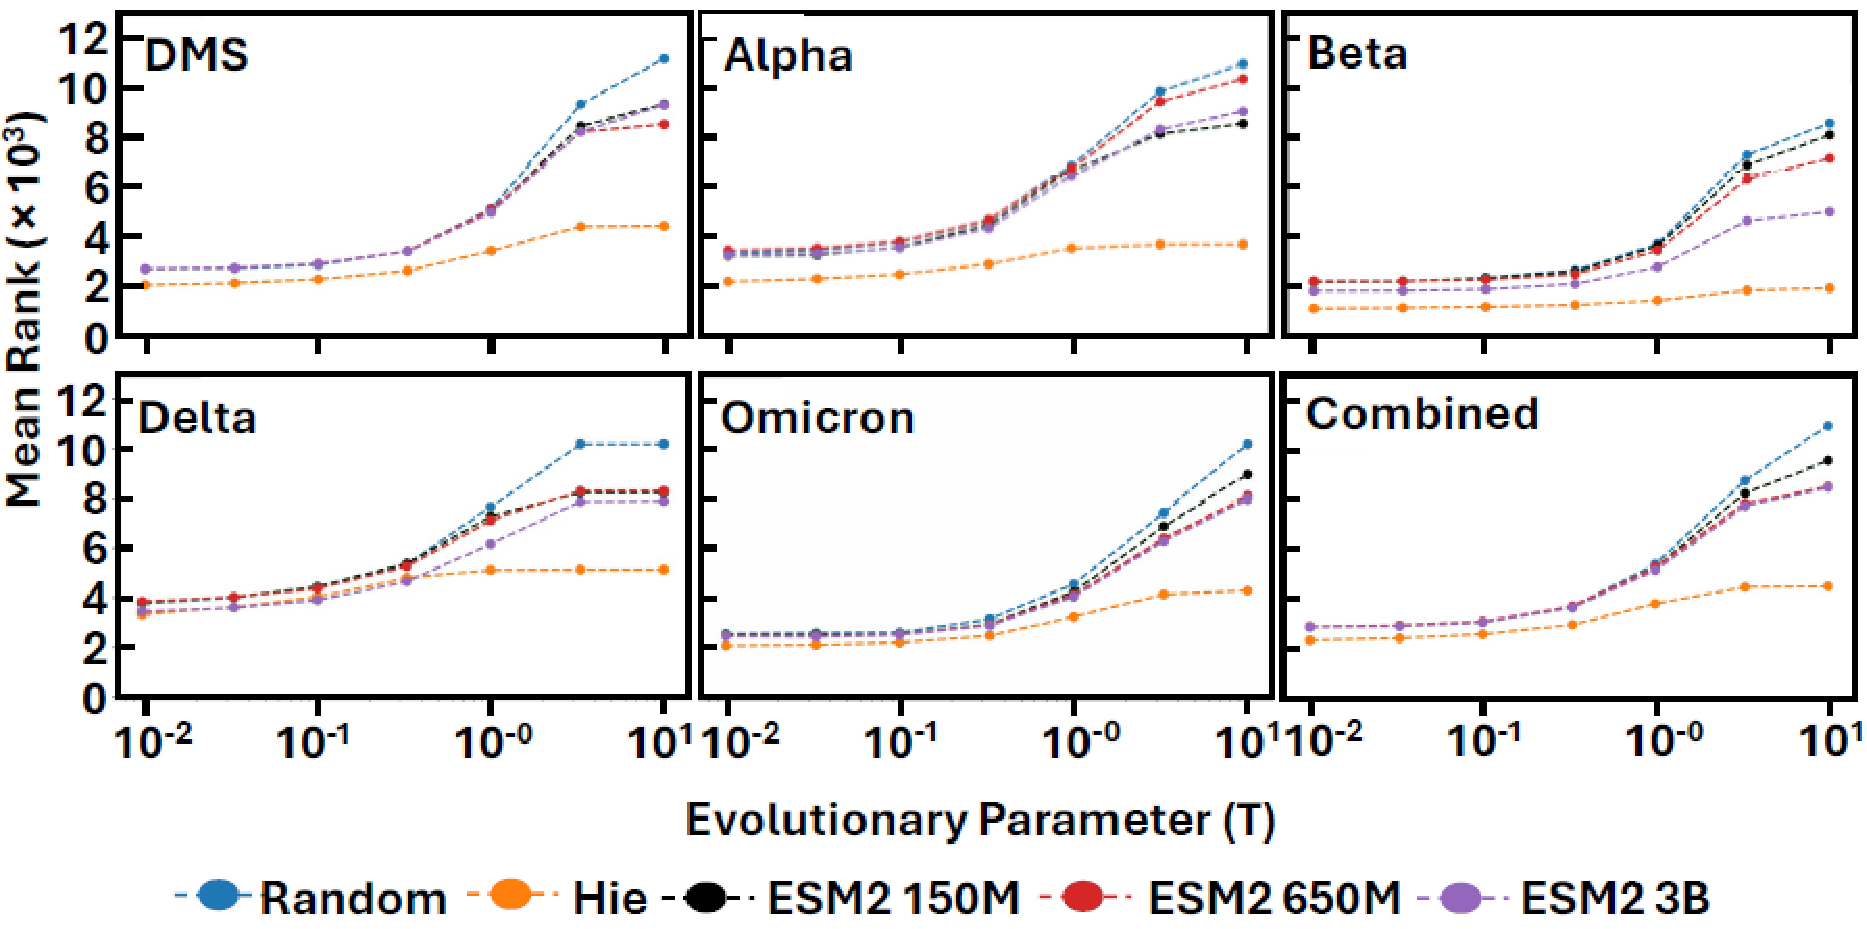
\includegraphics[width=\linewidth]{Figure_Nature_3.pdf}
    \caption{
    \textbf{Predictive performance is critically dependent on the evolutionary timescale.}
    Mean rank of known escape mutations from each validation set plotted as a function of the evolutionary timescale parameter, $T$ (horizontal axis, log scale).
    Each line represents a different PLM backbone.
    Panels correspond to different validation sets.
    Performance of the CAC is optimal at short timescales (small $T$) and decreases as $T$ increases.
    This highlights that near-term evolutionary events, which are strongly constrained by single-nucleotide accessibility, are most accurately captured by the model,
    while the influence of this constraint wanes over longer evolutionary periods.
}
    \label{fig:3}
\end{figure}

% The enhancement in CAC performance is largely due to the nucleotide-level information captured by the CLIMB regularizer, which is derived from SARS-CoV-2 mutational data~\cite{yi2021mutational}.
% To isolate this component, the ablation control group (CLIMB-only) use randomly generated semantic changes and grammaticality over 100 trials.
% Across these trials, it achieves a mean rank of 5100 $\pm$ 184 (grand mean $\pm$ SEM) in the DMS dataset.
% This result shows substantial predictive power, as the rank is less than half that of the negative control, 12012 $\pm$ 1588 (grand mean $\pm$ SEM).
% Notably, this performance well approaches that of the CSCS baseline using the Hie-BiLSTM (3757, mean rank) --- indicating that nucleotide mutation biases alone can be nearly as informative as the complete protein semantic model under these experimental conditions.

The performance gains of CAC are largely attributable to the nucleotide-level information captured by the CLIMB regularizer, inferred from SARS-CoV-2 mutational data~\cite{yi2021mutational}. To isolate this contribution, we evaluated an ablation in which candidate variants are ranked using only the CLIMB (mutation-process) term, while the semantic-change and grammaticality components are replaced with random scores (100 trials) to match the CAC scoring pipeline.

Across these trials, the CLIMB-only ablation achieves a mean rank of $5100 \pm 184$ (grand mean $\pm$ SEM) on the DMS dataset. This result shows substantial predictive power: the rank is less than half that of the negative control, $12012 \pm 1588$ (grand mean $\pm$ SEM). Notably, this performance approaches that of the CSCS baseline using the Hie-BiLSTM backbone (mean rank $3757$), indicating that nucleotide mutation biases alone can be highly informative under these experimental conditions.


\subsection*{Evolutionary timescale modulates the predictive strategy and component weights}

\begin{figure}[t]
    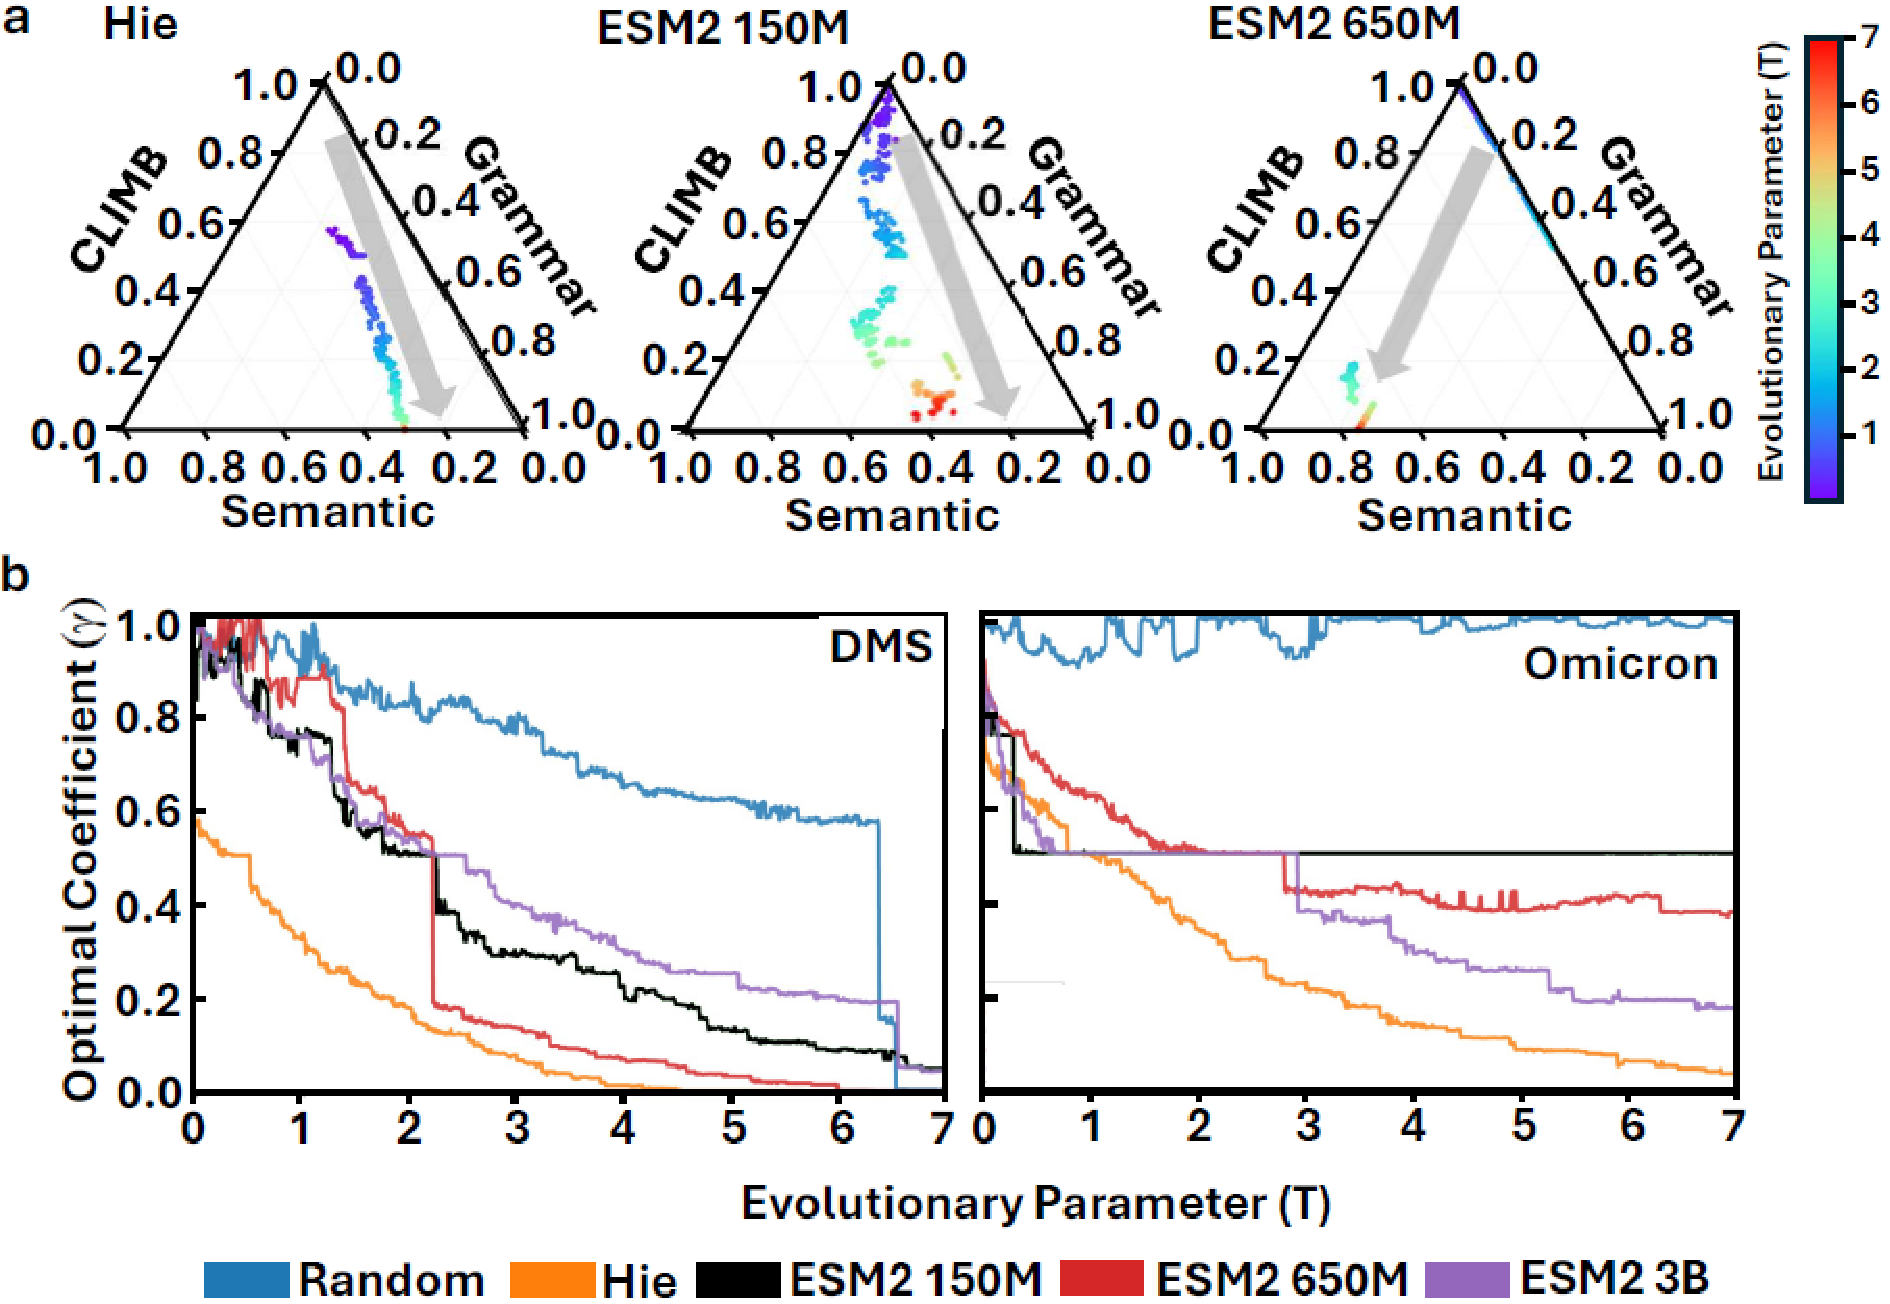
\includegraphics[width=\linewidth]{Figure_Nature_4.pdf}
    \caption{
    \textbf{Evolutionary timescale modulates the optimal weights of CAC components, revealing a dynamic predictive strategy.}
    %
    (\textbf{a}) Ternary plots illustrating the optimal weights $(\alpha, \beta, \gamma)$ that minimize the mean rank for each PLM backbone.
    These weights correspond to the contributions of semantic change ($s_s$), grammaticality ($s_g$), and the CLIMB regularizer ($s_p$), respectively.
    Each point represents an optimal weight combination for a specific evolutionary timescale $T$, colored by the value of $T$.
    The trajectory shows a systematic shift from the $\gamma$-vertex (CLIMB) towards the $\alpha$-$\beta$ edge (semantics/grammaticality) as $T$ increases.
    %
    (\textbf{b}) Optimal coefficient values for the CLIMB regularizer ($\gamma$) component plotted as a direct function of $T$ for the DMS validation set (left) and Omicron validation set (right).
    %
    The weight $\gamma$ is highest at small $T$ and systematically decreases.
    % This reveals a strategic trade-off between nucleotide-level accessibility and amino acid-level functional constraints over different evolutionary horizons.
}
    \label{fig:4}
\end{figure}

% The predictive strategy of the CAC method is critically modulated by the evolutionary timescale parameter, $T$, creating a trade-off between nucleotide-level mutational biases and learned protein-level functional rules.
% Our analysis reveals that overall predictive accuracy of the model is highest at smaller $T$ values --- it implies a strong reliance on near-term mutational likelihoods.
% For the Hie-BiLSTM model, the mean rank of the experimental group was lowest at $T=0.01$ ($2103$) and progressively increased to $4489$ at $T=10$ (Fig.~\ref{fig:3}).

% This strategic trade-off is directly reflected in the optimal weights of the model’s three components: (a) semantic change ($\alpha$), (b)  grammaticality ($\beta$), and (c) the CLIMB regularizer ($\gamma$) (Fig.~\ref{fig:4}).
% Over all the model backbones, the optimal contribution of the CLIMB component ($\gamma$) systematically decreases as $T$ increases.
% For example, using the Hie-BiLSTM model on the DMS dataset, the optimal $\gamma$ weight is $0.5372$ at $T=0.1$; but droppes to $0.0652$ at $T=3$.
% As the influence of the CLIMB regularizer wanes, the weights for semantic change ($\alpha$) and grammaticality ($\beta$) correspondingly increase.

% %This result confirms that
% We confirm that
% while near-term mutational likelihoods (small $T$) are highly predictive, the semantic and grammatical information from the PLM becomes indispensable for accurately ranking mutations over longer evolutionary periods.
% In these periods, nucleotide-level predictions are less certain.
The predictive strategy of CAC is critically modulated by the evolutionary timescale parameter, $T$, creating an explicit trade-off between nucleotide mutation biases (captured by CLIMB) and learned protein-level constraints (captured by the PLM semantic and grammatical scores). Consistent with Fig.~\ref{fig:3}, predictive accuracy is highest at small $T$, where short-horizon substitution tendencies dominate. For the Hie-BiLSTM backbone, the mean rank is lowest at $T=0.01$ ($2103$) and progressively increases to $4489$ at $T=10$ (Fig.~\ref{fig:3}).

This behavior is directly reflected in the optimal weights of the three components (Fig.~\ref{fig:4}). Across all backbones, the optimal CLIMB weight ($\gamma$) systematically decreases as $T$ increases, while the semantic-change ($\alpha$) and grammaticality ($\beta$) weights correspondingly increase. For example, using Hie-BiLSTM on the DMS dataset, the optimal $\gamma$ weight is $0.5372$ at $T=0.1$ but drops to $0.0652$ at $T=3$.

Together, these results indicate a clear time-scale--dependent shift: short-horizon prediction is driven primarily by the mutation-process prior (high $\gamma$), whereas at longer horizons the ranking increasingly relies on protein-level PLM constraints (higher $\alpha$ and $\beta$).


\subsection*{Codon-aware calibration reshapes the residue-level escape landscape}

% To assess the impact of codon-level constraints on SARS-CoV-2 immune escape prioritization, we calculate the change in the average escape rank for each residue ($\Delta\text{rank}$), where negative values signify a promotion to higher escape priority across four protein-language-model backbones --— Hie-BiLSTM, ESM-2-150M, ESM-2-650M, and ESM-2-3B (Fig.~5a). Domain-level means $\pm$ s.d.\ and all per-mutation values are listed in Table~S4.

% \begin{figure}[t]
%     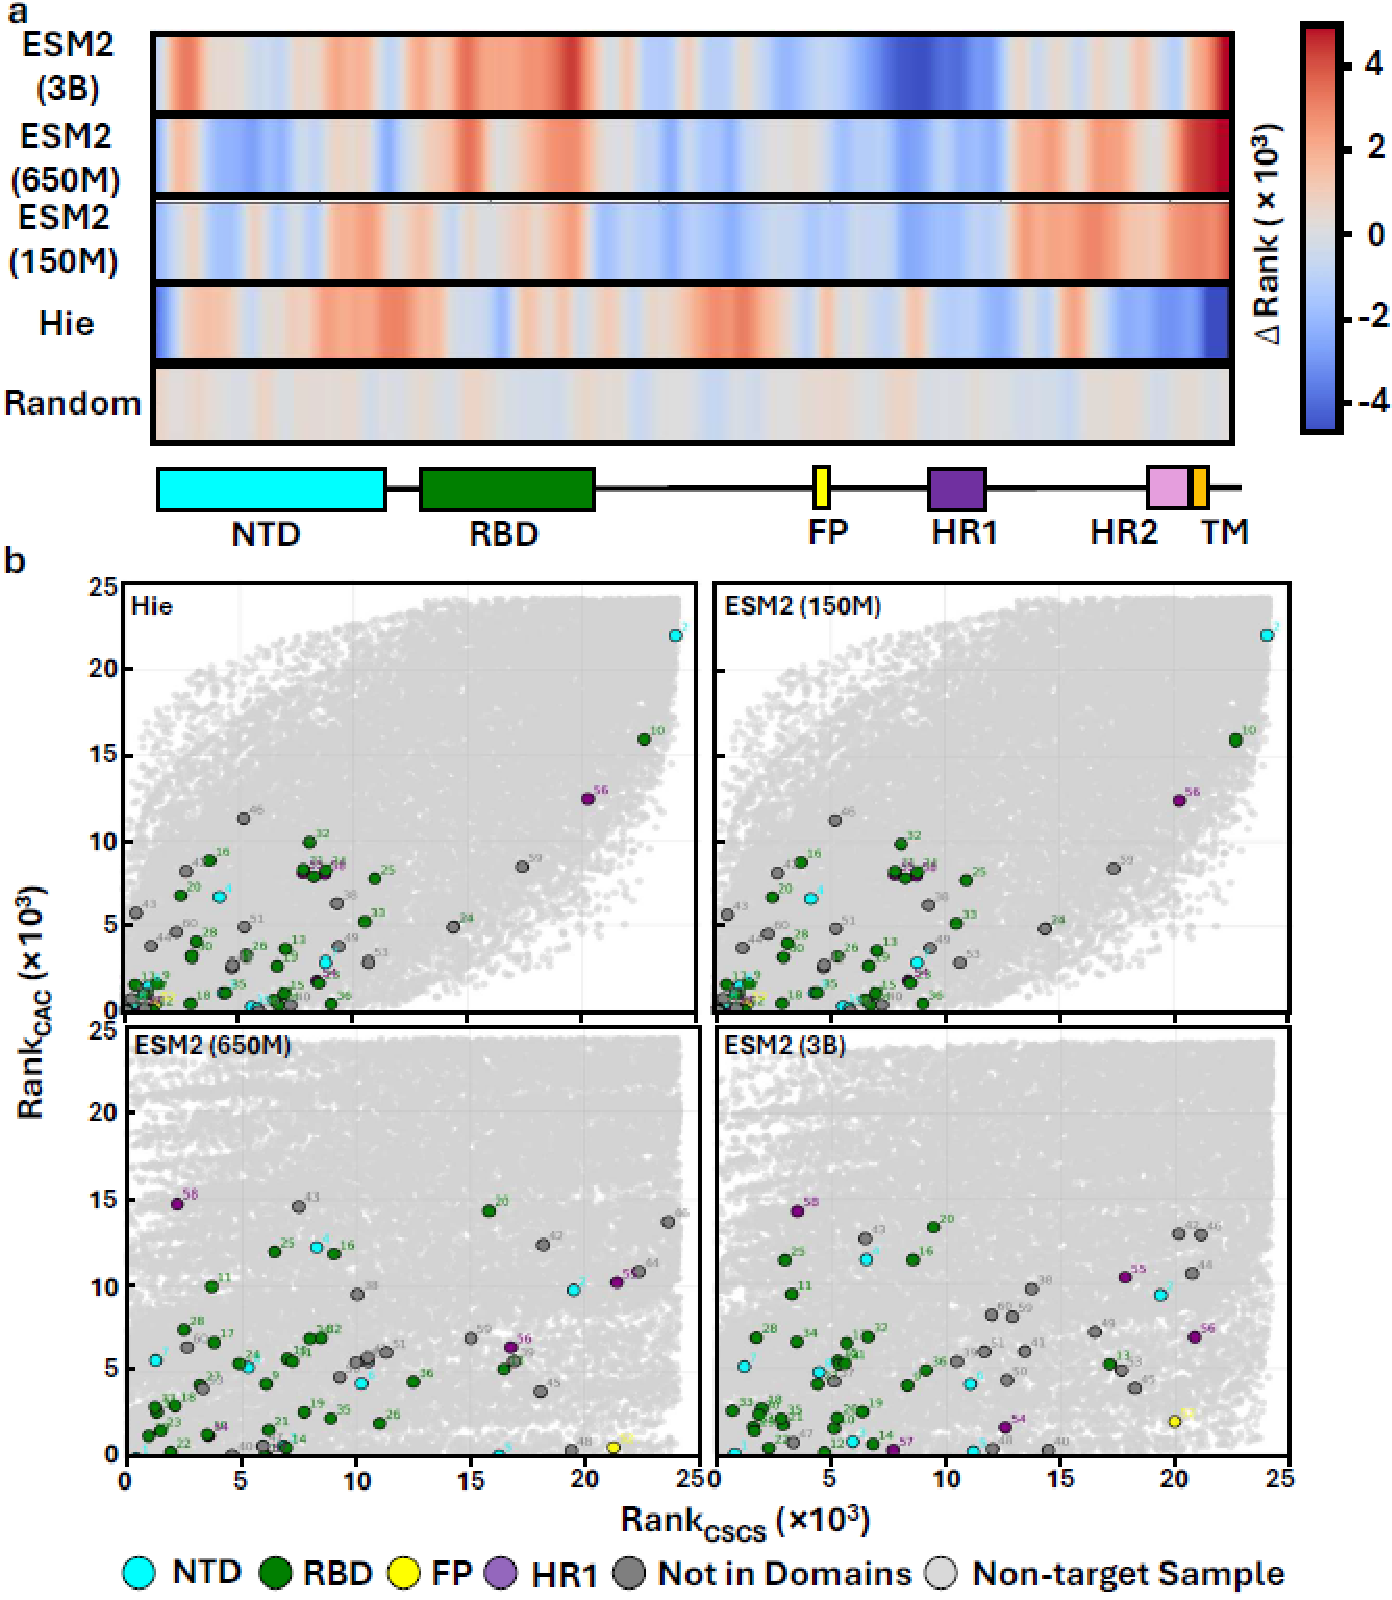
\includegraphics[width=\linewidth]{Figure_Nature_5.pdf}
%     \caption{\textbf{CAC selectively reshapes the SARS-CoV-2 spike escape landscape.}
%     %
%     (\textbf{a}) Heat map of mutation-rank shifts ($\text{rank}_{\text{CLIMB}} - \text{rank}_{\text{baseline}}$) for three protein-language-model backbones.
%     Negative values (blue) denote promotion to higher escape priority; positive values (red) denote demotion.
%     %
%     (\textbf{b}) Scatter plot comparing mutation ranks before (x-axis) and after (y-axis) CLIMB re-ranking for the 60 substitutions in the combined validation set.
%     The variants corresponding to each number are specified in Table S5. Domain boundaries are indicated above panels: N-terminal domain (NTD, residues 14--303), receptor-binding domain (RBD, 319--541), fusion peptide (FP, 788--806), heptad-repeat 1 (HR1, 912--984), heptad-repeat 2 (HR2, 1163--1213), and transmembrane helix (TM, 1214--1237) ~\cite{Winger2021Spike}.}
%     \label{fig:5}
% \end{figure}

% Domain escape priorities are reshaped by CAC in a backbone-dependent manner (Fig.~\ref{fig:5}a).
% Heptad-repeat~1 (HR1) gains priority across all backbones (overall range -852 to -4227; Table~S4).

% In contrast, the receptor-binding domain (RBD) is uniformly deprioritized (range 188 to 2598).
% The $N-$terminal domain (NTD) behaves inconsistently, gaining priority in the two smaller transformers (-451 and -956) but losing it in the BiLSTM and the largest transformer (883 and 525).
% The fusion peptide (FP) shows the opposite trend, rising in every transformer (-509 to -529) yet falling in the BiLSTM (1959).
% Heptad-repeat~2 (HR2) and the transmembrane domain (TM) climbs only in the BiLSTM (-2072 and -1856) and are penalized in all transformer backbones (+171 to +4131).
% These backbone-specific shifts confirm that CAC re-weights escape potential in a domain- and architecture-dependent fashion.

% Using the combined validation set, CAC promotes 45 of 60 variants with the ESM-2-150M backbone (75\%), outperforming ESM-2-650M (41/60, 68\%), ESM-2-3B (42/60, 70\%), and Hie-BiLSTM (40/60, 67\%) (Fig.~\ref{fig:5}b and Table S6).
% Domain-level inspection shows the highest recall for NTD in the 150M model (7/8 sites, 88\%) and the largest share of RBD substitutions jointly captured by Hie and 150M (18/28, 64\%), whereas the larger transformers trails (57--54\%).
% Crucially, all five HR1 sites are promoted in every backbone (5/5, 100\%).
% Thus, while some domains ---such as RBD--- display net demotion in the global analysis (Fig.~\ref{fig:5}a), CAC selectively elevated key escape sites within those domains, reprioritizing 64\% of RBD targets despite the overall downward shift and doing so without introducing novel variants.

To assess how the codon-transition prior reorders candidate substitutions across Spike, we quantify residue-level rank shifts induced by CAC relative to CSCS. Specifically, for each residue $i$ we compute
$\Delta \mathrm{rank}(i)=\langle \mathrm{rank}_{\mathrm{CAC}}-\mathrm{rank}_{\mathrm{CSCS}}\rangle$,
where the average is taken over all single-substitution candidates at residue $i$; negative values therefore denote promotion to higher escape priority. We evaluate these shifts across four backbones (Hie-BiLSTM, ESM2-150M, ESM2-650M, and ESM2-3B; Fig.~\ref{fig:5}a). Domain-level means $\pm$ s.d.\ and all per-mutation values are listed in Table~S4.

\begin{figure}[t]
    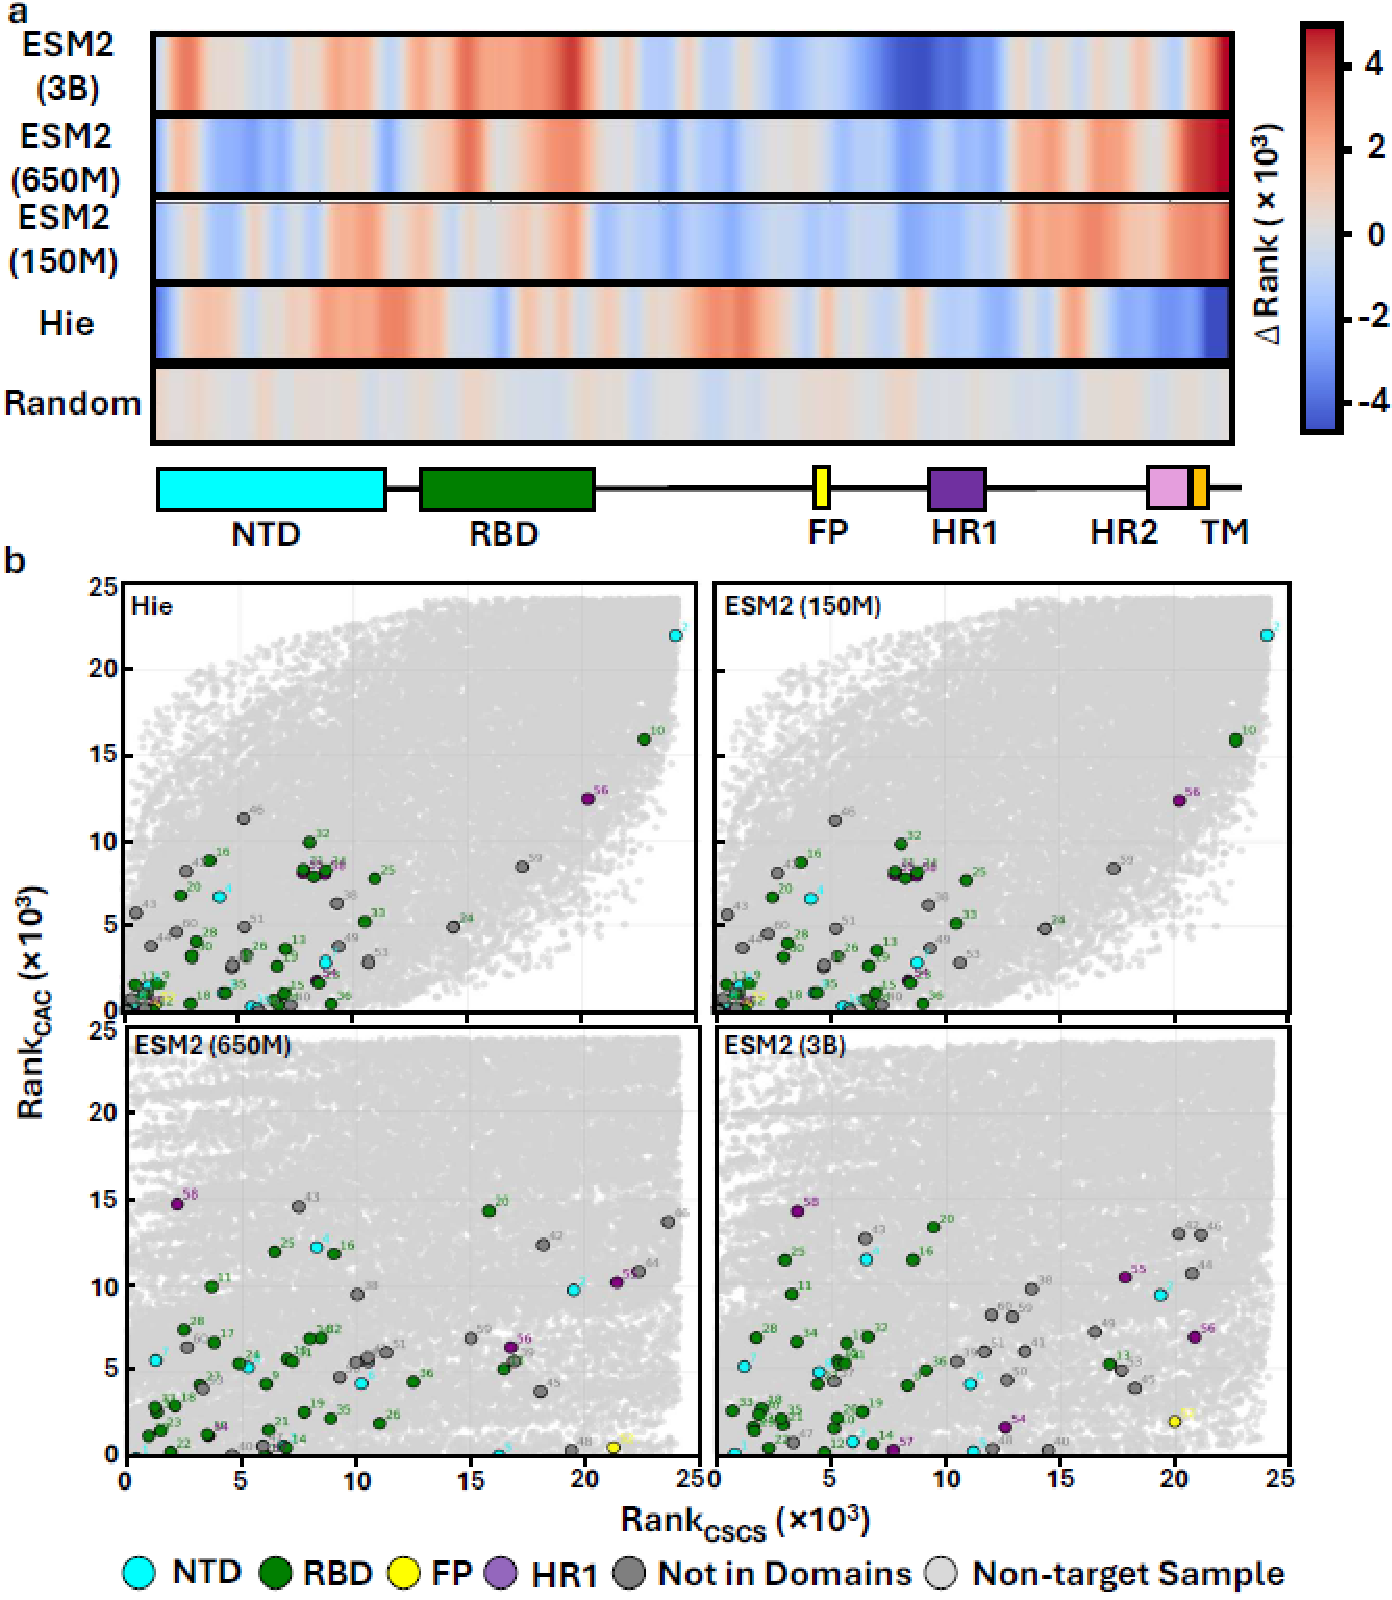
\includegraphics[width=\linewidth]{Figure_Nature_5.pdf}
    \caption{\textbf{CAC selectively reshapes the SARS-CoV-2 Spike escape landscape.}
(\textbf{a}) Heat map of mutation-rank shifts ($\mathrm{rank}_{\mathrm{CAC}} - \mathrm{rank}_{\mathrm{CSCS}}$) for three PLM backbones. Negative values (blue) denote promotion to higher escape priority; positive values (red) denote demotion.
(\textbf{b}) Scatter plot comparing mutation ranks before (x-axis; CSCS) and after (y-axis; CAC) re-ranking for the 60 substitutions in the combined validation set. The variants corresponding to each number are specified in Table S5. Domain boundaries are indicated above panels: N-terminal domain (NTD, residues 14--303), receptor-binding domain (RBD, 319--541), fusion peptide (FP, 788--806), heptad-repeat 1 (HR1, 912--984), heptad-repeat 2 (HR2, 1163--1213), and transmembrane helix (TM, 1214--1237)~\cite{Winger2021Spike}.}
    \label{fig:5}
\end{figure}

Domain escape priorities are reshaped by CAC in a backbone-dependent manner (Fig.~\ref{fig:5}a). Heptad-repeat~1 (HR1) gains priority across all backbones (overall range $-852$ to $-4227$; Table~S4). In contrast, the receptor-binding domain (RBD) is uniformly demoted in the global residue-level analysis (range $188$ to $2598$). The N-terminal domain (NTD) behaves inconsistently, gaining priority in the two smaller transformers ($-451$ and $-956$) but losing it in the BiLSTM and the largest transformer ($883$ and $525$). The fusion peptide (FP) shows the opposite trend, rising in every transformer ($-509$ to $-529$) yet falling in the BiLSTM ($1959$). Heptad-repeat~2 (HR2) and the transmembrane domain (TM) climb only in the BiLSTM ($-2072$ and $-1856$) and are penalized in all transformer backbones ($+171$ to $+4131$). These backbone-specific shifts indicate that the codon-transition prior interacts with backbone representations in a domain-dependent manner.

Using the combined validation set, CAC promotes 45 of 60 substitutions with the ESM2-150M backbone (75\%), outperforming ESM2-650M (41/60, 68\%), ESM2-3B (42/60, 70\%), and Hie-BiLSTM (40/60, 67\%) (Fig.~\ref{fig:5}b and Table S6). Domain-level inspection shows the highest recall for NTD in the 150M model (7/8 sites, 88\%) and the largest share of RBD substitutions jointly captured by Hie and 150M (18/28, 64\%), whereas the larger transformers trail (57--54\%). Crucially, all five HR1 sites are promoted in every backbone (5/5, 100\%). Thus, while some domains---such as RBD---exhibit net demotion in the global residue-level summary (Fig.~\ref{fig:5}a), CAC selectively elevates key escape targets within those domains, reprioritizing 64\% of RBD targets despite the overall downward shift, within the same single-substitution candidate set considered by CSCS.


\section*{Discussion}

We show that incorporating a codon-transition prior into amino-acid--level semantic scoring substantially improves viral escape prioritization across multiple protein language model (PLM) backbones and validation settings. Conceptually, CAC addresses a systematic \emph{model--process mismatch}: existing PLM-based approaches evaluate candidate variants in protein space, while the generative mechanism that produces variation is governed by a nucleotide-level mutation process. By injecting mutation-process information as an explicit, separately weighted term, CAC augments amino-acid--only objectives with a feasibility prior grounded in codon transitions \cite{Halpern1998, Rodrigue2010}. Importantly, this correction is implemented \emph{post-hoc} and is therefore model-agnostic, requiring neither retraining nor access to backbone internals. This property is especially relevant in modern forecasting pipelines that increasingly rely on large, frozen foundation models.

A central computational insight of CAC is that the optimal combination of process-level and protein-level signals depends on the evolutionary horizon. Varying the time-scale parameter $T$ reveals a systematic shift in the optimal weights: at short horizons (small $T$), prediction relies more strongly on the CLIMB term, whereas at longer horizons the contribution of CLIMB decreases and the PLM-derived semantic and grammatical components dominate. Rather than treating $T$ as an incidental hyperparameter, CAC makes it an interpretable control knob that modulates how strongly the scoring objective is regularized by the mutation process. This horizon-dependent mixture provides a unified view of ranking across regimes: near-term prediction is bottlenecked by mutation-process plausibility, while longer-horizon ranking increasingly reflects compatibility with protein-level constraints learned by the PLM.

CAC builds on the constrained semantic change framework of Hie et al.~\cite{hie2021learning} by explicitly incorporating nucleotide-level information that is typically omitted in amino-acid--only objectives. In our experiments, the specialized Hie-BiLSTM backbone frequently performs competitively and sometimes outperforms general-purpose ESM-2 backbones on single-substitution benchmarks. We view this observation primarily as a \emph{methodological} point about evaluation and representation: (i) training data specificity may provide an advantage for certain viral tasks, and (ii) architectural inductive biases can affect how a model responds to isolated point substitutions versus distributed sequence constraints. Rather than interpreting these differences as definitive statements about biological mechanisms, CAC makes such backbone-dependent behaviors explicit and measurable, facilitating systematic comparison of forecasting pipelines.

Beyond aggregate accuracy, CAC reshapes residue- and domain-level rank summaries in a structured way. From a computational perspective, these shifts are best interpreted as consequences of reweighting the scoring objective: adding a codon-transition prior redistributes priority toward substitutions favored under the inferred mutation process, and this redistribution can interact with backbone representations. As a result, coarse domain-level averages can show net demotion even when many validated targets within the same domain are promoted. This highlights an important point for practical use: landscape visualizations should be treated primarily as \emph{diagnostics of model behavior} and as tools for hypothesis generation, not as standalone biological conclusions.

Our results also suggest an engineering implication: because backbone representations and their interaction with the codon-transition prior can differ, combining multiple backbones may yield more robust rankings by reducing sensitivity to any single model's inductive biases \cite{Botz2024dynamic}. In this sense, CAC can serve as a common calibration interface for ensemble forecasting: different PLMs can be compared and combined under a shared process-aware objective, with explicit weights that enable auditing and horizon-specific tuning.

Several limitations motivate future extensions. First, CLIMB is parameterized from an empirical mutation spectrum that may shift across time, lineages, or environments; a prior inferred from one regime may become miscalibrated in another. This motivates stratified estimation, adaptive updating, and uncertainty-aware weighting of the process term. Second, our current evaluation focuses on single substitutions, whereas longer-term evolution often involves multi-step trajectories and epistatic interactions. Extending CAC from single-step codon transitions to path-based likelihoods, and incorporating explicit models of combinatorial effects, would better support long-horizon scenario generation. Third, CLIMB is intentionally lightweight; richer process priors---including context-dependent nucleotide models, synonymous constraints, and host-specific translational efficiency measures (e.g., tAI/CAI)---could be integrated as additional modular terms without modifying PLM backbones \cite{Plotkin2010Synonymous, Shao2024Riboformer, Wu2024Genome, Rapino2021Wobble, Zhang2023Algorithm}.

Overall, CAC provides a portable, post-hoc calibration layer that corrects a fundamental model--process mismatch in amino-acid--only PLM predictors. By coupling general-purpose protein-level representations with an explicit codon-transition prior, CAC improves escape prioritization, exposes an interpretable horizon-dependent trade-off, and offers a practical template for integrating mechanistic process knowledge into black-box foundation-model pipelines for biological forecasting.

% \section*{Discussion}

% %Our study
% We demonstrate that
% integrating codon transition probabilities with protein-level semantic models substantially improves the accuracy and biological interpretability of viral evolution prediction.
% This finding establishes a unified framework for modeling viral adaptation, in which the distinct ``languages'' of codons and amino acids are considered in unison.
% To accurately forecast an evolutionary trajectory, one must account for both the genetic probability of a mutation occurring (the codon language) and the functional permissibility of its outcome (the amino acid language)\cite{Halpern1998, Rodrigue2010} .

% The balance between these two languages is not static but shifts depending on the evolutionary context, a phenomenon revealed by the analysis of the time parameter~$T$.
% For short-term evolution (small~$T$), predictions rely heavily on the CLIMB regularizer.
% We interpret this as reflecting the early adaptive dynamics where readily accessible single-point mutations are the primary drivers of escape, making their genetic probability highly predictive.
% However, as~$T$ increases, the predictive influence of the CLIMB regularizer wanes.
% This likely signifies a shift in the evolutionary landscape, where the cumulative impact of combinatorial (multi-point) mutations becomes more critical for significant antigenic change than any single, genetically probable mutation.

% This work builds upon the foundational concept of Hie et al.~\cite{hie2021learning} by incorporating the missing layer of nucleotide-level information and creating a more complete predictive framework.
% An interesting result is that the specialized Hie-BiLSTM model generally outperformed the larger generalist ESM-2 models in our CAC framework, particularly in metrics like mean rank and AUC.

% We propose this stems from two primary factors.
% First is training data specificity; the Hie model was trained on a curated corpus of viral proteins, potentially allowing it to learn the specific ``dialect'' of viral evolution more effectively.

% Second, and more consequentially, are the architectural differences between the models.
% The sequential processing of a BiLSTM is inherently specialized for evaluating the impact of a single amino acid change within its local context.
% This structural focus likely explains its superior performance in our experimental setup, which is confined to predicting the effects of single point mutations.
% In contrast, transformer models, with their global self-attention mechanism, are designed to capture complex and long-range dependencies across the entire sequence.
% While this led to lower predictive accuracy for isolated point mutations, this global perspective
% %appears to have
% has induced a more significant and biologically relevant re-ranking of mutational risk across distant structural domains.
% There are observed in our analysis of the S1 and S2 subunits~\cite{hie2021learning, Alley2019, Rao2019, Rao2021MSA, Meier2021}.

% Our improved predictive framework yield crucial biological insights into SARS-CoV-2 spike protein evolution.
% It demonstrates % and support
% how a mutation's likelihood of emergence is primarily governed by codon accessibility rather than by domain identity alone~\cite{Gunnarsson2023Predicting, Cano2022Mutation, Lauring2012Codon}.
% %
% Even within domains under strong selective pressure, such as the receptor-binding domain (RBD), codon-hotspots persist where mutations can occur with minimal genetic cost. This highlights that local sequence context can override global structural constraints in guiding viral evolution.
% As a consequence, vaccine antigens designed to simply mask the entire RBD may be insufficient~\cite{Letscher2025RBD, Huang2020Structural}; instead immunogen design should focus on stabilizing these specific permissive patches.
% %Although the
% S2 subunit is highly conserved across sarbecoviruses~\cite{Guenthoer2024S2, Guo2023Targetable};
% our CAC nevertheless uncovers differential mutational opportunities, with its HR1 region becoming more favorable.
% This finding strongly demonstrates that high sequence identity within the fusion-peptide and HR1 regions does not preclude adaptive evolutionary pathways.
% Thus, it underscores the critical need for continuous surveillance of these S2 elements to pre-empt antibody escape and steer next-generation vaccine design~\cite{Pang2022variant, Lei2023Functional,Chen2022Broadly, Park2023SARS, Hsieh2024Prefusion, Guo2023Targetable}.

% Beyond these specific biological findings, our study reveals that model architecture significantly influences the perceived vulnerability of viral proteins with distinct rank shifts observed between models like Hie and ESM-2.
% It emphasizes that ensemble modeling across diverse architectures could provide more robust forecasts of viral escape by mitigating biases from any single model~\cite{Botz2024dynamic}.

% For countermeasure development, the utility of our CAC framework is substantial: it effectively raises the ranking of mutations already observed in patients without generating new as well as unobserved sequences.
% Since it makes a valuable addition to genomic surveillance pipelines for flagging variants with high evolutionary feasibility.

% Additionally, the insights gained from CAC suggest the design of structure-guided vaccines that stabilize these identified permissive sites in both the RBD and HR2, thereby effectively limiting the virus’s mutational capacity and narrowing the scope for future immune escape.
% % In essence,
% Incorporating CAC into routine monitoring offers a powerful, orthogonal filter for assessing mutational risk and significantly enhances our preparedness for the continuing evolution of SARS-CoV-2.

% Our framework provides a significant advance; it also opens several avenues for
% %future
% refinement.
% %
% The mutational spectrum data used to parameterize CLIMB represent a snapshot from a specific period of the pandemic and may itself evolve.
% %Furthermore, as noted,
% As noted, our current model focuses on the effects of single point mutations.
% %A crucial next step
% It is meaningful to devise methods capable of evaluating the
% combinatorial effects of multiple mutations, which often drive major evolutionary leaps.
% In parallel with advancing models that account for combinatorial mutations,
% %future research may also
% it is also beneficial
% from integrating codon-level biological priors into amino-acid–based predictive pipelines.
% For example, codon-aware features --—such as synonymous-degeneracy, wobble-base usage, and host-specific translational efficiency measures like the tRNA Adaptation Index (tAI) or Codon Adaptation Index (CAI)---
% %can
% possibly
% provide orthogonal information on genetic accessibility~\cite{Plotkin2010Synonymous, Shao2024Riboformer, Wu2024Genome, Rapino2021Wobble, Zhang2023Algorithm}.
% As shown in our CAC analysis, such features
% %would improve
% would be meaningful in enhancing
% prioritization performance across diverse PLMs and could facilitate a more unified two-language framework for modeling viral evolution.


\section*{Materials and methods}\label{sec:methods}

\subsection*{CSCS}%{Constrained Semantic Change Search}

First we review the concept of CSCS introduced by Hie et al.~\cite{hie2021learning}, which quantifies the likelihood of viral escape due to point mutations using embeddings of amino acid sequences in a latent space.

% \subsubsection{Definition of the CSCS score}
An amino acid sequence is represented as a sequence $\mathbf{a} = (a_1, a_2, \dots, a_N) \in \mathcal{A}^N$, where $\mathcal{A}$ is the standard amino acid alphabet and $N$ is the length of the sequence. Each possible single amino acid substitution from $a_i$ to $\tilde{a}_i$ at position $i$ will be indicated as $a_i \to \tilde{a}_i$, and the resulting mutated sequence from $\mathbf{a}$ is denoted as $\mathbf{a}[\tilde{a}_i]$.

A semantic embedding is a mapping that encodes each amino acid sequence $\mathbf{a} \in \mathcal{A}^N$ into a vector $\mathbf{z}$ in a latent space $\mathbb{R}^k$.
Ideally, sequences with similar biological properties are embedded close together.
Then the semantic change ($\mathrm{s}_\text{s}$) caused by the mutation $a_i \to \tilde{a}_i$ is measured by the similarity between the respective embeddings $\mathbf{z}$ and $\mathbf{z}[\tilde{a}_i]$ of the original sequence~$\mathbf{a}$ and mutated sequence~$\mathbf{a}[\tilde{a}_i]$ using a prescribed similarity function $d : \mathbb{R}^k \times \mathbb{R}^k \to \mathbb{R} $:
\begin{align}
    \mathrm{s}_\text{s}
    \triangleq d(\mathbf{z}, \mathbf{z}[\tilde{a}_i]).
    \label{e:sc_theory}
\end{align}

The grammaticality ($\mathrm{s}_\text{g}$) of the mutation $a_i \to \tilde{a}_i$ is defined as the likelihood of observing amino acid $\tilde{a}_i$ at position $i$ given the rest of the sequence $\mathbf{a}_{[N]\setminus\{i\}}$.
Ideally, this probability is higher if the mutated sequence $\mathbf{a}[\tilde{a}_i]$ is grammatically consistent with the protein language and lower otherwise.
%
Under the assumption that all semantic information of $\mathbf{a}_{[N]\setminus\{i\}}$ is retained in its embedding vector, denoted~$\mathbf{z}_i$, the grammaticality can be computed as:
\begin{align}
    \mathrm{s}_\text{g}
    \triangleq
    p(\tilde{a}_i \mid \mathbf{z}_i).
    %p(\tilde{a}_i \mid \mathbf{a}_{[N]\setminus\{i\}}).
    \label{e:g_theory}
\end{align}

%In~\cite{hie2021learning},
The authors of Hie-BiLSTM model~\cite{hie2021learning} posited that both high semantic change and high grammaticality help better predict viral escape and introduce a ranking method, termed CSCS, that prioritizes mutations exhibiting these characteristics.
More concretely, given the sequence~$\mathbf{a}$, the ranking of the single amino acid substitutions is based on the CSCS score defined as:
\begin{align}
    \mathtt{CSCS}(\tilde{a}_i)
    \triangleq
    f_\text{s}(\mathrm{s}_\text{s}) + f_\text{g}(\mathrm{s}_\text{g}),
    \label{e:cscs_theory}
\end{align}
where $f_\text{s}$ and $f_\text{g}$ are increasing transformations for the values of semantic change $\mathrm{s}_\text{s}$ and grammaticality $\mathrm{s}_\text{g}$, respectively. For instance, the version of the CSCS score in~\cite{hie2021learning} employs ranking transforms for $f_\text{s}$~and~$f_\text{g}$.

\subsection*{Biological model for single-base substitution}
We define a model for single-base substitutions that occur during the spread and viral escape of SARS-CoV-2 and outline the method for identifying model parameters from data.

% \subsubsection{Model definition}
Our model posits that the assumption of the standard substitution model holds in the phylogenetic tree of SARS-CoV-2 genomes~\cite{felsenstein2003inferring}. Let $\mathcal{B} = \{ \mathsf{A}, \mathsf{C}, \mathsf{G}, \mathsf{U} \}$ represent the set of all possible nucleotide bases.
The assumption asserts that the phylogenetic tree of viral evolution can be described as an instance of a branching Markov process on the space $\mathcal{B}^N$ of genomes of fixed length $N$, where single-base substitutions at each position occur independently of other positions and depend solely on the current base at that position.

%More specifically,
We model the phylogenetic tree as the union of all observed lineages of viral genomes starting from the wildtype genome at time $t = 0$. Each observed lineage is represented as the sample path of a continuous-time stochastic process $\mathbf{b}_t \in \mathcal{B}^N$ that undergoes a series of single-base substitutions.
Here, $t$ denotes the time elapsed since the initial observation of the wildtype genome.
Under the standard substitution model assumption, the base $b_t \in \mathcal{B}$ at a given specific position in $\mathbf{b}_t$ evolves according to a continuous-time Markov process on $\mathcal{B}$ with the transition rate matrix:
\begin{align}
    \mathbf{Q} = [q_{uv}]_{u,v \in \mathcal{B}}.
\end{align}
%
Here, each off-diagonal transition rate $q_{uv}$ is a positive number representing the average rate at which base $u$ mutates to base $v$. The diagonal entries $q_{uu}$ are defined such that (i) each row $u$ of the matrix $\mathbf{Q}$ sums to zero, i.e., $q_{uu} = -\sum_{v\neq u} q_{uv}$, and that (ii) the average rate of substitutions of any type per unit time is $1$.

% \subsubsection{Parameter estimation}
To estimate $\mathbf{Q}$, we first construct a phylogenetic tree from sequence alignment data.
We then count $n_{uv}$, the number of observed single-base substitutions of type $u \to v$ across all branches, and $n_u$, the total number of base $u$ across all positions and sequences.
Then the estimator $\hat{q}_{uv}$ for the transition rate $q_{uv}$, for $u \neq v$, is computed using the following formula:
\begin{align}
    \hat{q}_{uv} = \frac{n_{uv} / (\sum_{u' \neq v'} n_{u'v'})}{n_u / (\sum_{u'} n_{u'})}.
\end{align}


%
\subsection*{Codon-aware prediction model for viral escape}

% For a complete document, you would need \documentclass{article} and packages like \usepackage{amsmath}
% This is a snippet intended for inclusion in a larger document.

%Here,
We now introduce a new term to improve the CSCS method.
%
The original grammaticality score, $\mathrm{s}_\text{g}$~\eqref{e:g_theory}, assesses the fitness of a mutation conditioned on the surrounding sequence, but it omits the original amino acid $a_i$.
In the context of predicting viral escape, this omission can introduce a selection bias by ignoring nucleotide-level information from the wildtype codon at position~$i$, such as its mutational susceptibility.
We hypothesize that the predictive power of CSCS can be improved by incorporating this nucleotide-level evolutionary information.
To test this, we suggest the CLIMB regularizer.

Specifically, we augment the original CSCS score~\eqref{e:cscs_theory} with an additional term, the CLIMB regularizer ($\mathrm{s}_\text{p}$).
%
This term represents the likelihood of a new amino acid~$\tilde{a}_i$ occurring at position~$i$ after an elapsed time~$T$, given the wildtype codon~$\mathbf{c}$.
The value of this regularizer is computed as:
\begin{align}
    \mathrm{s}_\text{p}
    \triangleq p_T(\tilde{a}_i \mid \mathbf{c})
    &=
    \sum_{\tilde{\mathbf{c}} \mathop{:} \begin{subarray}{c}
        \text{codon} \\ \text{for $\tilde{a}_i$}
    \end{subarray}}
    \prod_{k=1}^{3} [\mathrm{e}^{T\mathbf{Q}}]_{c_k, \tilde{c}_k}.
    \label{e:CLIMB}
\end{align}
Here, $\mathbf{c} = (c_1, c_2, c_3) \in \mathcal{B}^3$ is the $i$-th codon of the wildtype genome, and the sum runs over all possible codons~$\tilde{\mathbf{c}}$ for the amino acid~$\tilde{a}_i$.

We then redefine the CSCS score by incorporating this regularizer.
The resulting score, CAC, is given by:
\begin{align}
    \mathtt{CAC}(\tilde{a}_i)
    \triangleq
    f_\text{s}(\mathrm{s}_\text{s}) + f_\text{g}(\mathrm{s}_\text{g})
    + f_\text{p}(\mathrm{s}_\text{p}),
    \label{e:cscs_reg}
\end{align}
where $f_\text{p}$ is an increasing transformation for the CLIMB regularizer~$\mathrm{s}_\text{p}$.

\subsection*{Models and datasets}

%\subsubsection{Protein Language Models}


We calculate the semantic change ($\mathrm{s}_\text{s}$) and grammaticality ($\mathrm{s}_\text{g}$) scores using several PLMs pre-trained on a masked language modeling task.
%
For a given amino acid sequence, we first extract its embedding vector and the model's positional output probabilities.
Specifically, the embedding of the entire sequence is defined as the output from the final representation layer (i.e., the last LSTM layer for BiLSTM models or the last transformer layer for transformer models).
The grammaticality score at a specific position is derived from the softmax output probabilities at that position.

The models used in this study includes the BiLSTM from Hie~et~al.~\cite{hie2021learning} and three models from the ESM-2 family: ESM-2-150M, ESM-2-650M, and ESM-2-3B~\cite{lin2023evolutionary}.
%
Using these models, we generate scores for all possible single-nucleotide and non-synonymous substitutions relative to a given reference sequence.
The calculation of semantic change ---defined as the similarity between embedding vectors--- is model-dependent: we use the $\ell^1$-distance for the Hie-BiLSTM model and cosine similarity for the ESM-2 models.

%\subsubsection{Nucleotide Substitution Data for CLIMB}
The CLIMB regularizer ($\mathrm{s}_\text{p}$) is calculated using SARS-CoV-2 single-nucleotide variant frequency data sourced from Yi et al.~\cite{yi2021mutational}.
This dataset provides single-base substitution counts categorized into 192 subclasses based on flanking 5' and 3' nucleotides, which we use to estimate the transition rate matrix $\mathbf{Q}$.
(Further details of this computation are provided in the Supplementary Information.)

We implement the CAC score with a specific choice of transformations:
\begin{align}
    \mathtt{CAC}
    = \alpha \cdot \mathtt{z}(\mathrm{s}_\text{s})
    + \beta \cdot \mathtt{z}(\log \mathrm{s}_\text{g})
    + \gamma \cdot \mathtt{z}(\log \mathrm{s}_\text{p}).
    \label{e:cscs_reg_impl}
\end{align}
%
Here, $(\alpha, \beta, \gamma)$ are barycentric weights satisfying $\alpha, \beta, \gamma \geq 0$ and $\alpha + \beta + \gamma = 1$, which are chosen to ensure optimal performance.
The function~$\mathtt{z}$ standardizes its input variable $\mathrm{s}$ to have zero mean and unit variance across all possible non-synonymous single-base substitutions in the reference spike protein sequence.
%
Note that the grammaticality ($\mathrm{s}_\text{g}$) and CLIMB scores ($\mathrm{s}_\text{p}$) are log-transformed prior to standardization, as log-likelihood provides a natural measure of information content.

%\subsubsection{Validation Data}
The performance of CAC is evaluated against multiple, distinct sets of experimentally verified and lineage-defining mutations.
The primary validation set comprises 19 ground-truth escape mutations for the Wuhan-Hu-1 wild-type reference sequence (NCBI accession: NC\_045512.2) as identified by the DMS data from Baum et al.~\cite{baum2020antibody}.

To further assess the model's predictive power on evolved strains, we construct additional validation sets using the characteristic point mutations of four major variants of concern.
These variants, their respective reference sequences, and the number of characteristic mutations used for validation are:
Alpha (MZ344997.1, 7~mutations), Beta (MZ433432.1, 8~mutations), Delta (OK091006.1, 7~mutations), and Omicron (BA.1, OL672836, 30~mutations).
The validation process is conducted independently for each of these datasets.

%
%
\subsection*{Performance evaluation}

% \subsubsection{Experimental Design and Groups}
Our experimental design involve comparing four distinct configurations for each PLM (BiLSTM, ESM-2-150M, ESM-2-650M, and ESM-2-3B).
The primary configuration under investigation is the experimental group, representing our full model \eqref{e:cscs_reg_impl} that combines semantic change, grammaticality, and the CLIMB regularizer.

This is evaluated against three control groups:
(a) the standard control group, consisting of the original CSCS method using only semantic change and grammaticality as the primary baseline,
(b) an ablation control group, which combined the CLIMB regularizer with randomly generated semantic and grammaticality scores to isolate the independent predictive power of our nucleotide-level contribution, and
(c) a negative control group based solely on randomly generated scores for all components to establish random-chance performance levels.

% \begin{figure}[h]
%     \centering
%     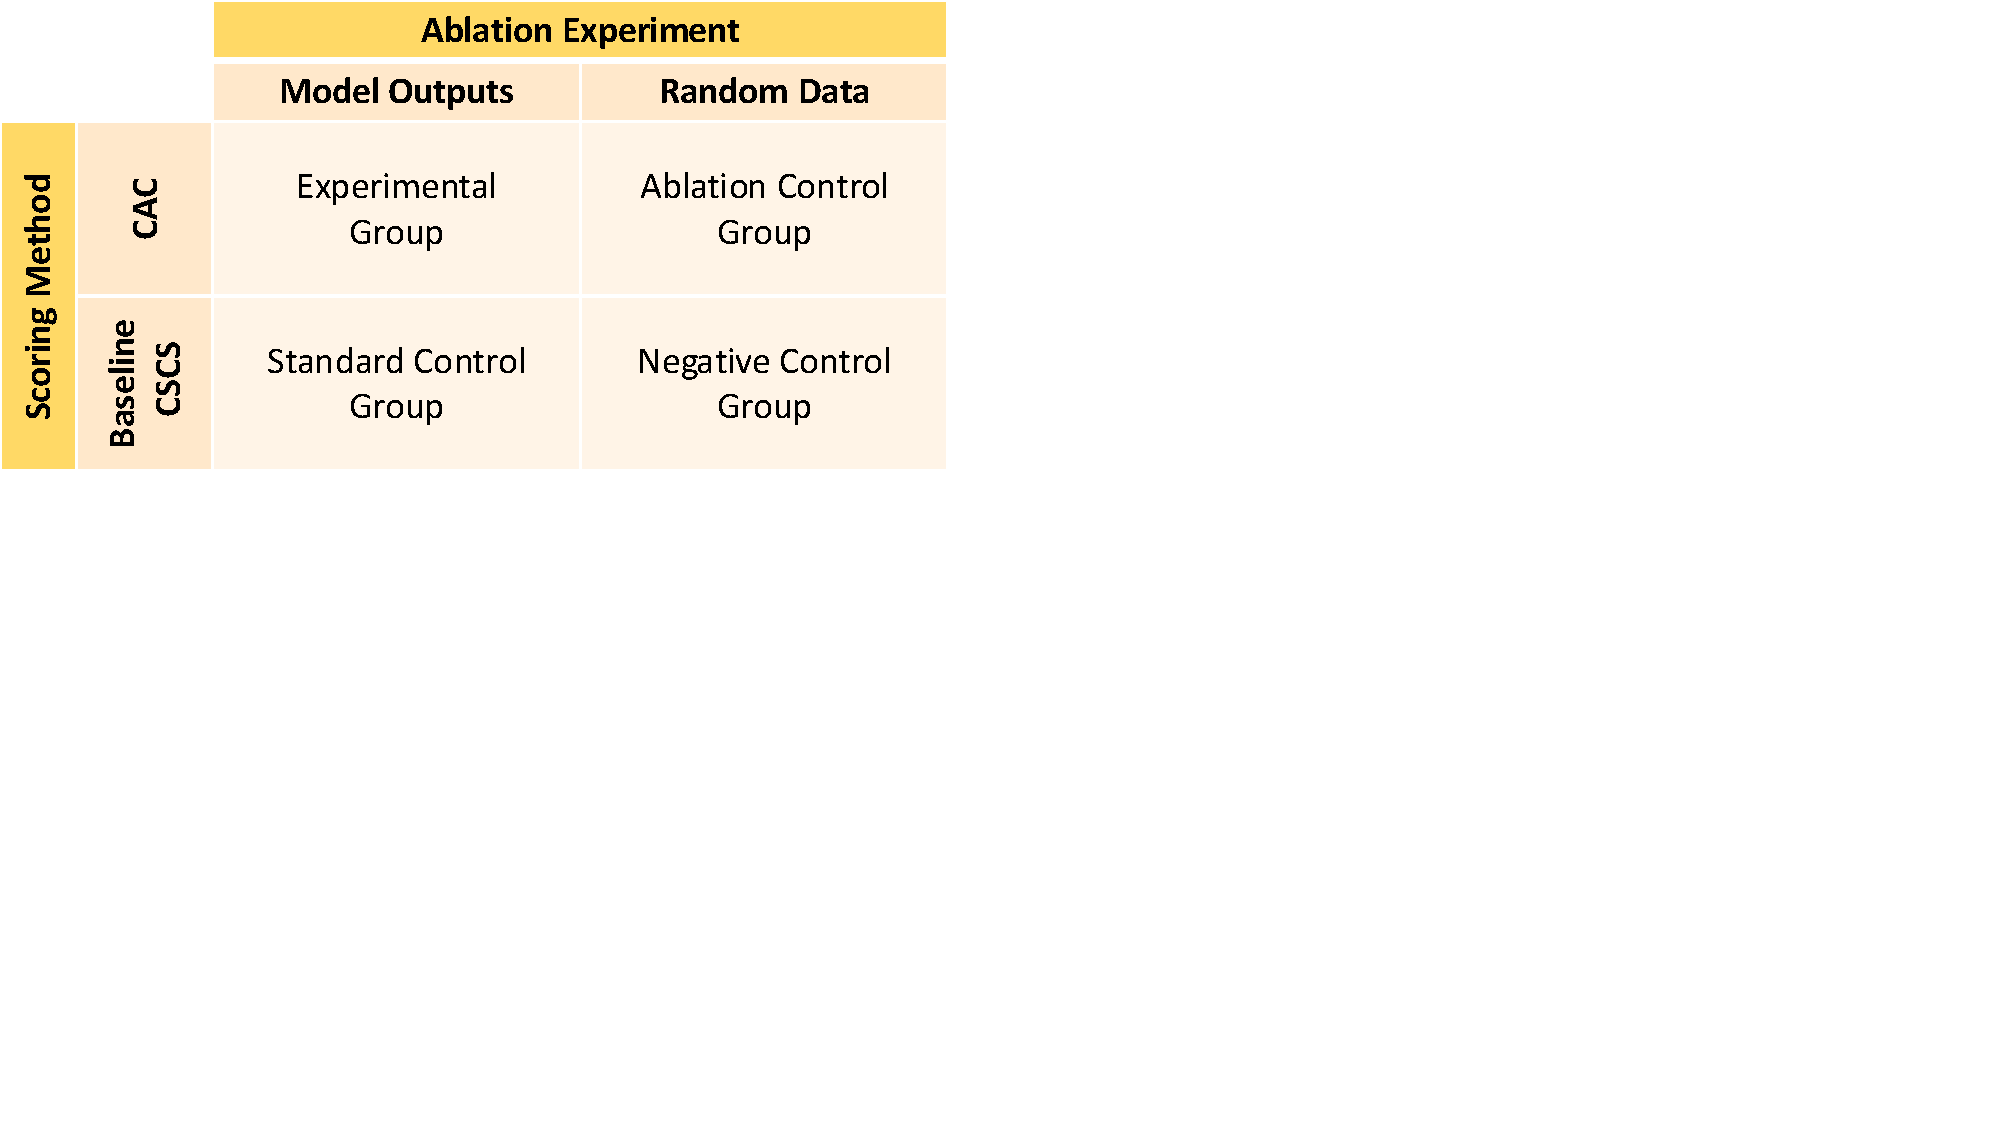
\includegraphics[width=0.9\linewidth]{table_1.pdf}
% \end{figure}

% \subsubsection{Metrics and Analysis}
The performance of each group is well quantified using two primary metrics: the area under the curve (AUC) and the mean rank of the true validation mutants among all 24,187 possible non-synonymous point mutations on the wild-type spike protein sequence.
The specific values for these metrics are provided in the Supplementary Information.
To intuitively summarize and compare the performance across groups, we visualize the distribution of ranks for the validation mutants using box-and-whisker plots, in which each contains a five-number summary.

We further investigate the impact of the time parameter $T$ in the CLIMB regularizer by evaluating CAC's performance across a range of values ($0.01$, $0.033$, $0.1$, $0.33$, $1$, $3.3$, $10$).
%Furthermore
Moreover,
to understand the dynamic interplay between the CAC components,
%we visualize
the optimal coefficients $(\alpha, \beta,$ and $ \gamma)$ are visualized on a ternary plot.
This is achieved by calculating the optimal coefficients that minimized the mean rank for 1,000 discrete values of $T$ spanning from 0.001 to 7.
The analysis is repeated for each combination of protein model and validation set.


\section*{Acknowledgements}
%We thank the AI/R Lab sequencing team for helpful discussions.
This work is supported by grant Nos.
2023-00262155 (AIDE); 2024-00460980 (deFAI); 2025-02304717 ((AI)$^2$) (all from IITP), and
%NRF‑
2025R1A5A1031234; 2021R1A2C1095046 (all from NRF)
funded by the Korea government (the Ministry of Science and ICT).
%and
RS-2023-00266133 (the Korea Health Technology R$\&$D Project) also supports this work.
Additionally, we are also grateful to the KIST's institutional grants for their support.
%supported
%by the KIST's institutional grants.

\section*{Code availability}
All source code developed for this study is publicly available on GitHub (\url{https://github.com/sos440/climb}) and has been permanently archived on Zenodo (DOI: \href{https://doi.org/10.5281/zenodo.15744443}{10.5281/zenodo.15744443}).

\section*{Data availability}
All data generated and analyzed during this study, including calculated codon-aware constrained semantic change search (CAC) scores and model component scores, are publicly available on Zenodo (DOI: \href{https://doi.org/10.5281/zenodo.15744443}{10.5281/zenodo.15744443}). The datasets used for model validation and parameterization were obtained from previously published public resources; accession numbers for reference sequences are provided in the Materials and methods.

\section*{Author contributions}
H.J., D.Y., and S.L.\ contributed equally to this work and investigated the work overall. H.J., D.Y., and S.L.\ wrote the original manuscript with input from all authors. H.J.\ and D.Y.\ prepared datasets, curated data, and tested various baseline models. S.L.\ proposed and developed the mathematical/statistical modeling and performed statistical analyses based on formal analyses of S.L.\ and D.Y. S.L.\ and D.Y.\ also evaluated the performance of the model. H.J.\ and S.L.\ developed the software and performed computational analyses. H.C.\ revised the software, conceived, and edited the manuscript. C.J.\ and C.K.\ conceived, conceptualized, led the project, revised and edited the manuscript, and acquired funding. C.K.\ supervised all aspects of the research.

\section*{Competing interests}
The authors declare no competing interests.

\bibliography{sn-bibliography}

% \printbibliography

\end{document}
